\chapter{Theoretische Achtergrond}
\label{hst-theorie}
Dit hoofdstuk bevat de theoretische concepten die nodig zijn om de gebruikte aanpak zo goed mogelijk te begrijpen. Het bevat een beschrijving van de gebruikte neurale netwerken en van een aantal concepten uit de statistiek.

\section{Neurale Netwerken}
Algemeen gesproken dient een neuraal netwerk als een simulatie van menselijke hersenen. De structuur van een neuraal netwerk probeert de werking van de neuronen en synapsen in het menselijke brein na te bootsen. Neuronen zijn de primitieve eenheden van het menselijke zenuwstelsel. Ze staan in verbinding met elkaar en communiceren met elkaar door middel van elektrische potentiaal. Afhankelijk van de aan- of afwezigheid van potentiaal over de inkomende verbindingen stuurt een neuron al dan niet een signaal door naar het volgende neuron. Deze eenheden zijn zeer makkelijk softwarematig te simuleren.
Elk artificieel neuraal netwerk heeft een trainingsfase nodig waarin het de juiste gewichten leert. Na deze training kan het netwerk ongeziene input omvormen tot de juiste output.


Deze sectie geeft een inleiding tot de gebruikte neurale netwerken. Een eerste deel handelt over het eenvoudigste type neuraal netwerk (feedforward), dat de basis vormt voor een aantal gebruikte varianten. Daarna volgt een toelichting van enkele meer complexe netwerken: recurrente en convolutionele neurale netwerken, alsook Long Short Term Memory netwerken.

\subsection{Feed Forward Neurale Netwerken}
\paragraph{Perceptron} % (fold)
\label{par:perceptron}

Om een feedforward neuraal netwerk te begrijpen is het concept perceptron nodig. Dit is een netwerk bestaande uit een of meer neuronen, met een of meerdere inputs ($x_i$). De output $y$ van een neuron is een gewogen som van alle inputs met gewichten $w_i$, al dan niet gewijzigd met een transferfunctie $f$ (formule \ref{formule:neuron}). Typische voorbeelden van transferfuncties zijn de logistische functie en de hyperbolische tangensfunctie.

\begin{equation}
    y = f(\sum\limits_{i=1}^{n}w_i x_i)
    \label{formule:neuron}
\end{equation}

Het is ook mogelijk om een perceptron met meerdere outputs te gebruiken. Hierbij heeft elke input \'e\'en gewicht per output en kan elke output een verschillende transferfunctie hebben. Figuur \ref{fig:perceptron} toont een perceptron met vijf inputs en drie outputs. Deze architectuur komt exact overeen met drie aparte neuronen die allemaal dezelfde inputs krijgen, maar elk verschillende gewichten en een verschillende transferfunctie $f_i$ gebruiken.

\begin{figure}[ht]
\def\layersep{2.5cm}
\centering
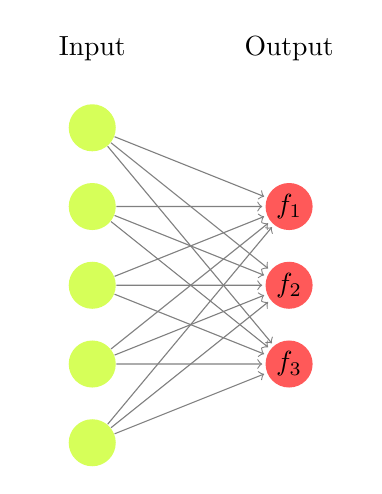
\begin{tikzpicture}[shorten >=1pt,->,draw=black!50, node distance=\layersep]
    \tikzstyle{every pin edge}=[<-,shorten <=1pt]
    \tikzstyle{neuron}=[circle,fill=black!100,minimum size=17pt,inner sep=0pt]
    \tikzstyle{input neuron}=[neuron, fill=lime!65];
    \tikzstyle{output neuron}=[neuron, fill=red!65];
    \tikzstyle{annot} = [text width=4em, text centered]

    %input neurons
    \foreach \name / \y in {1,...,5}
        \path[yshift=0.5cm]
            node[input neuron] (I-\name) at (0,-\y cm){};

    %output neurons
    \foreach \name / \y in {1,...,3}
        \node[output neuron] (O-\name) at (\layersep,-\y-0.5) {$f_{\name}$};

    %links
    \foreach \source in {1,...,5}
        \foreach \dest in {1,...,3}
            \path (I-\source) edge (O-\dest);

    % Annotate the layers
    \node[annot,above of=I-1, node distance=1cm] (i1) {Input};
    \node[annot,right of=i1] (hl2) {Output};
\end{tikzpicture}
\caption{Perceptron met vijf inputs en drie outputs}
\label{fig:perceptron}
\end{figure}


\paragraph{Feedforward Netwerk}
\label{par:concept}
Een feedforward neuraal netwerk is een van de eenvoudigste neurale netwerken. Het is een perceptron met \'e\'en of meer verborgen lagen tussen input en output. De outputs van elke laag worden enkel doorgegeven aan de volgende laag, er zijn dus geen cycli in het netwerk (zie figuur \ref{fig:ffnn}). Elke pijl op de figuur vertegenwoordigt een vermenigvuldiging met een bepaald gewicht. Het is voor elke knoop in het netwerk ook mogelijk om een transferfunctie te gebruiken alvorens de waarde door te sturen naar de volgende laag. Hier is het ook mogelijk om een outputlaag te gebruiken met meerdere knopen, wat neerkomt op een parallelle uitvoering van meerdere netwerken met een enkele output.\cite{Bishop:1995:NNP:525960} Daarnaast hoeft een knoop niet alle outputs van een vorige laag te gebruiken. Wanneer het niet volledig verbonden is, komt dit immers neer op een gewicht van 0 voor de niet-verbonden knopen.

\begin{figure}[ht]
\def\layersep{2.5cm}
\centering
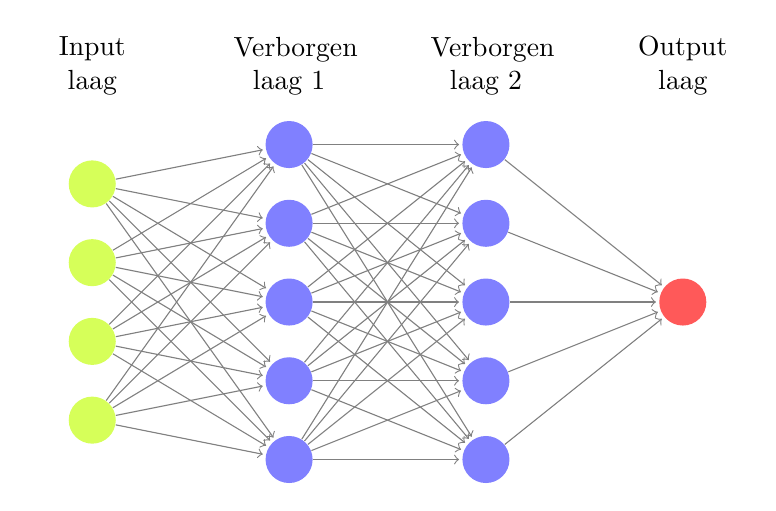
\begin{tikzpicture}[shorten >=1pt,->,draw=black!50, node distance=\layersep]
    \tikzstyle{every pin edge}=[<-,shorten <=1pt]
    \tikzstyle{neuron}=[circle,fill=black!25,minimum size=17pt,inner sep=0pt]
    \tikzstyle{input neuron}=[neuron, fill=lime!65];
    \tikzstyle{output neuron}=[neuron, fill=red!65];
    \tikzstyle{verborgen neuron}=[neuron, fill=blue!50];
    \tikzstyle{annot} = [text width=4em, text centered]

    % Draw the input layer nodes
    \foreach \name / \y in {1,...,4}
    % This is the same as writing \foreach \name / \y in {1/1,2/2,3/3,4/4}
        \node[input neuron] (I-\name) at (0,-\y) {};

    % Draw the hidden layer nodes
    \foreach \name / \y in {1,...,5}
        \path[yshift=0.5cm]
            node[verborgen neuron] (H1-\name) at (\layersep,-\y cm) {};

    % Draw the hidden layer nodes
    \foreach \name / \y in {1,...,5}
        \path[yshift=0.5cm]
            node[verborgen neuron] (H2-\name) at (2*\layersep,-\y cm) {};

    % Draw the output layer node
    \node[output neuron, right of=H2-3] (O) {};

    % Connect every node in the input layer with every node in the
    % hidden layer.
    \foreach \source in {1,...,4}
        \foreach \dest in {1,...,5}
            \path (I-\source) edge (H1-\dest);
    %links van eerste naar tweede hidden layer
    \foreach \source in {1,...,5}
        \foreach \dest in {1,...,5}
            \path (H1-\source) edge (H2-\dest);

    % Connect every node in the hidden layer with the output layer
    \foreach \source in {1,...,5}
        \path (H2-\source) edge (O);

    % Annotate the layers
    \node[annot,above of=H1-1, node distance=1cm] (hl1) {Verborgen laag 1};
    \node[annot,above of=H2-1, node distance=1cm] (hl2) {Verborgen laag 2};
    \node[annot,left of=hl1] {Input laag};
    \node[annot,right of=hl2] {Output laag};
\end{tikzpicture}
\caption{Feedforward Neuraal Netwerk met twee verborgen lagen}
\label{fig:ffnn}
\end{figure}

% paragraph concept (end)

\paragraph{Training} % (fold)
\label{par:training}
Het trainen van een feedforward netwerk gebeurt meestal met terugpropagatie. Deze techniek vergelijkt de verwachte output bij een gekende input met de berekende output. Op basis van dit verschil gebeuren er aanpassingen aan de gewichten in omgekeerde richting: eerst de gewichten van de laatste laag, dan de voorlaatste, \ldots 

Voor een netwerk met \'e\'en verborgen laag geldt het volgende voor de waarden van de verborgen knopen $\mathbf{\hat{h}}$ en voorspelde outputvector $\mathbf{\hat{y}}$ bij inputvector $\mathbf{x}$:
\begin{equation}
    \mathbf{\hat{h}} = f(\mathbf{Wx})
\end{equation}
\begin{equation}
    \boldsymbol{\hat{y}} = f(\boldsymbol{W'\hat{h}}) = f(\boldsymbol{\hat{h}'}) = f(\boldsymbol{W'}f(\boldsymbol{Wx}))
\end{equation}
waarbij $\mathbf{W}$ en $\mathbf{W'}$ de gewichten van de verbindingen tussen respectievelijk de input en de verborgen laag, en de verborgen laag en de output voorstellen. $f$ is telkens de transferfunctie. In deze formule is ze gelijk voor elke laag, maar het is mogelijk om voor elke laag een andere functie te gebruiken.

Het probleem bij het leren van $\mathbf{W}$ en $\mathbf{W'}$ is dat de correcte verborgen vector $\mathbf{h}$ niet gekend is. De training van het netwerk kan dus enkel op basis van de input,de  berekende output en de verwachte output gebeuren.

Een eerste stap is het verkleinen van het verschil $\mathbf{\hat{y}} - \mathbf{y}$ door het aanpassen van \myvector{W'} en \myvector{\hat{h}}. \myvector{W'} wordt gewijzigd met behulp van gradient descent, veronderstellende dat \myvector{\hat{h}} correct is. Gradient descent is een eenvoudig optimalisatie algoritme dat kan dienen om het lokale minimum van een functie te vinden. De minimalisatie gebeurt op een ``gulzige'' manier, door elke stap wijzigingen aan te brengen in de richting van de steilste afdaling. Deze richting komt overeen met de eerste afgeleide van de transferfunctie, berekend in alle variabelen van de output van het netwerk: 

\begin{equation}
df_i = \frac{d}{d\hat{h_i}'}f(\hat{h_i}')
\end{equation}
In het geval van een logistische transferfunctie $f(x) = \frac{1}{1 + \mathrm e^{-x}}$ geeft dit volgende vector van afgeleiden:
\begin{equation}
  \mathbf{df} = \frac{d}{d\hat{h}'}\mathbf{\hat{y}} = \mathbf{\hat{y}}(1-\mathbf{\hat{y}})
\end{equation}

De formule om de gewichten te updaten ziet er in het algemene geval uit als volgt:
\begin{equation}
  w'_{ji} = w'_{ji} + \sigma(y_j-\hat{y}_j)df_i\hat{h}_i
\end{equation}
Hierbij stelt $\sigma$ de leersnelheid (learning rate) voor. De leersnelheid bepaalt hoe zwaar de aanpassing aan de gewichten doorweegt.
Indien er een logistische transferfunctie wordt gebruikt geeft dit het volgende resultaat:
\begin{equation}
    w'_{ji} = w'_{ji} + \sigma(y_j-\hat{y}_j)\hat{y}_j(1-\hat{y}_j)\hat{h}_i
\end{equation}
Elke stap zorgt deze gradient ervoor dat aanpassing van de gewichten ervoor zorgt dat, bij dezelfde input, de output dichter bij het gewenste resultaat zal liggen.

Vervolgens zorgt gradient descent voor een aanpassing van \myvector{\hat{h}}. Er kunnen echter geen wijzigingen worden aangebracht in \myvector{\hat{h}} zelf, dus wijzigt het algoritme \myvector{W} zodat de fout op \myvector{\hat{h}} het meeste verkleint. Gradient descent leidt tot volgende \myvector{\Delta h}, die de gewenste verandering van \myvector{\hat{h}} weergeeft:
\begin{equation}
    \Delta h_i = \sum\limits_{j}(y_j-\hat{y}_j)\hat{y}_j(1-\hat{y}_j)w'_{ji}
\end{equation}
Op basis van \myvector{\Delta h} en \myvector{\hat{h}} kan \myvector{W} gewijzigd worden met volgende formule:
\begin{equation}
    w_{ji} = w_{ji} + \sigma(\Delta h_j)\hat{h}_j(1-\hat{h}_j)x_i
\end{equation}

\todo{boek van blockeel quoten}

Op deze manier verkleint de fout op de output \myvector{\hat{y}-y}, deels door de verandering in \myvector{W} en deels door die in \myvector{W'}.
Deze techniek wordt toegepast voor elk paar van gekende inputs en outputs zodat kleine wijzigingen op termijn de juiste gewichten leren. Het is ook mogelijk om elke input meerdere keren toe te passen op het netwerk. Deze methode kan bovendien eenvoudig worden uitgebreid naar een netwerk met een arbitrair aantal verborgen lagen. Hierbij propageert de fout van elke laag door naar de gewichten van de vorige laag. Een zelfde techniek maakt het trainen mogelijk van complexere structuren met terugkoppelingen (RNN) of convolutionele lagen (CNN).
% paragraph training (end)

\paragraph{Softmaxlaag}\label{par:softmax}
De softmaxlaag is een laag die vaak als laatste laag in een neuraal netwerk voorkomt. Wanneer het netwerk meerdere outputs heeft, geeft de softmaxlaag een kansverdeling over de verschillende outputs terug in plaats van de oorspronkelijke outputvector. Concreet betekent dit dat de outputwaarden worden genormaliseerd op een manier dat elke waarde positief is en bovendien de som van alle waarden gelijk is aan 1. Dit is bijvoorbeeld nuttig bij het leren van een kansverdeling over een aantal discrete componenten. Ook bij classificatie van input die tegelijkertijd tot meerdere klassen kan behoren is dit van nut.
In het geval van onze thesis komt een softmax voor als laatste laag bij de gebruikte CNN, als laatste laag in het netwerk om de topicverdeling te bepalen bij een LDA en als laatste laag in het gebruikte taalnetwerk.\todo{refereren naar secties?} \todo{afgeleide ook uitleggen voor backprop + formule}

De softmaxlaag is eigenlijk de softmaxfunctie in formule \ref{formula-softmax}. Hierbij is $o$ de outputvector van grootte $n$.
\begin{equation}
softmax(o)_i = \frac{e^{o_i}}{\sum^{n}_{k=1}{e^{o_k}}}
\label{formula-softmax}
\end{equation}


% CNN
\subsection{Convolutionele Neurale Netwerken}
\label{sec:CNN}
Convolutionele Neurale Netwerken (ConvNets of CNN's) zijn een biologisch ge\" inspireerde trainbare architecturen die invariante afbeeldingskarakteristieken kunnen leren.\cite{LeCun2010} Ze bieden een hi\"erarchische representatie van een afbeelding en zijn van nut in tal van visuele taken.\cite{Girshick2014}\cite{Ciresan2012}\cite{Zhou2015}

Een CNN is een \emph{deep learning} architectuur bestaande uit verschillende niveaus. De input en output van elk niveau is een verzameling van arrays die men een \emph{feature map} noemt. Op elke output is de feature map een representatie van een bepaald kenmerk van de afbeelding. Elk niveau bestaat standaard uit drie lagen: een filter bank laag, een non-linearity laag en een feature pooling laag. Na een aantal van deze niveaus is er nog een classificatielaag.\todo{types lagen verder uitdiepen?}

Eerst is er een filter bank laag, die een aantal features kan detecteren in de input. Daarna volgt een niet-lineaire laag. Deze kan een eenvoudige functie bevatten zoals een sigmo\"ide of de $\tanh$ functie, maar kan ook veel complexer zijn en bijvoorbeeld een ``rectified sigmoid'' bevatten, al dan niet gecombineerd met een normalisatie. \todo[inline]{meer schrijven over deze lagen } De laatste laag in het niveau is een feature pooling laag die de dimensionaliteit van de output reduceert door regio's van de output te vervangen door hun gemiddelde of maximumwaarde.

Trainen van dit netwerk kan gesuperviseerd met behulp van terugpropagatie, maar ook zeer snel ongesuperviseerd waardoor er geen nood is aan zeer grote gelabelde datasets. CNN's zijn in staat om veel sneller concepten te leren dan gewone feedforward netwerken, terwijl ze theoretisch slechts iets mindere resultaten kunnen bekomen. Een CNN gebruikt op elk niveau rechthoekige regio's uit de vorige laag die bovendien mogen overlappen. Door deze overlapping is het netwerk translatie-invariant.

E\'en van de meest succesvolle toepassingen van CNN's is objectdetectie. Deze vooruitgang was vooral te wijten aan een paper\cite{Krizhevsky2012a} die CNN's gebruikt voor het oplossen van de ImageNet challenge.\cite{Russakovsky2014}
Dit is een competitie waarin afbeeldingen moeten worden geclassificeerd in een aantal voorgedefini\"eerde categorie\"en. De gebruikte architectuur bestaat uit 8 lagen waarvan 5 convolutioneel en 3 volledig verbonden. Ze gebruiken bovendien verschillende technieken om overfitten te vermijden. Als classificatielaag gebruiken ze softmax zodat het netwerk een kansverdeling over de verschillende categori\"een leert. De architectuur kan worden gezien in figuur \ref{fig:AlexNet} en  is een variant op de standaardarchitectuur die hierboven werd beschreven. Dit netwerk was het best presterende netwerk voor de wedstrijd in 2012. Ondertussen zijn nog diepere architecturen voorgesteld die op dezelfde en recentere wedstrijden nog betere resultaten bekomen.

Het netwerk (VGGNet)\cite{Arge2015} dat wij gebruiken bestaat uit 16 lagen en is publiek beschikbaar met behulp van Caffe\cite{Jia2014}. De feature maps van verschillende outputlagen van dit netwerk dienen als input voor andere taken dan de ImageNet Challenge. Zo kan de output van de laatste laag voor de classificatielaag worden beschouwd als een representatievector voor de hele afbeelding. Output van de andere lagen is een representatie voor afbeeldingskenmerken op een niveau lager dan de volledige afbeelding.
\begin{figure}[tb]
	\centering
	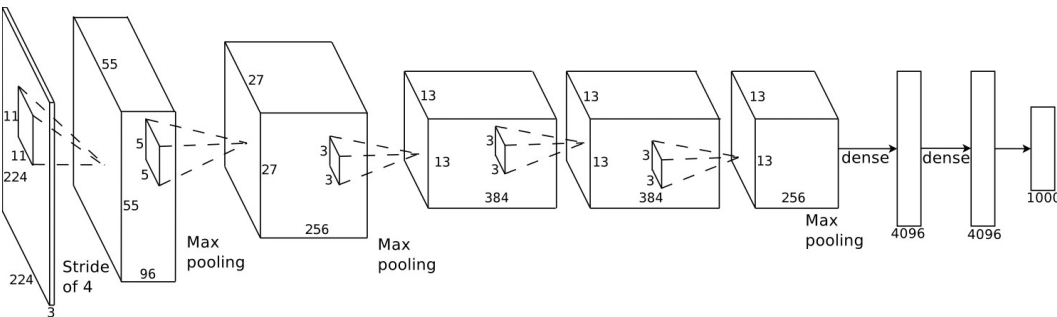
\includegraphics[width=\linewidth]{Images/cnn.PNG}
	\caption{Convolutioneel Neuraal Netwerk gebruikt door \cite{Krizhevsky2012a} voor classificatie van afbeeldingen}
	\label{fig:AlexNet}
\end{figure}

% RNN
\subsection{Recurrente Neurale Netwerken}
\todo[inline]{we hebben buiten word2vec geen enekele referentie in dit stuk?}
Recurrente neurale netwerken zijn een uitbreiding van standaard feedforward neurale netwerken. Ze kunnen, net zoals feedforward netwerken, getraind worden met terugpropagatie. Het grote verschil met feedforward netwerken is de terugkoppeling van de output van de vorige stap naar de verborgen lagen. Op figuur \ref{fig:rnn} \todo{reference voor afbeeldng + meer uitleg over wat een ontrolling is} is een ontrolling van een RNN over verschillende tijdstippen te zien. $U,V$ en $W$ stellen gewichtsmatrices voor.

De terugkoppeling zorgt ervoor dat het netwerk in staat is om informatie te onthouden. Hierdoor kunnen recurrente netwerken tijdsgerelateerde informatie coderen. Daarom zijn ze geschikt om sequenti\"ele data, zoals tekst, te modelleren en te voorspellen. Recurrente neurale netwerken kunnen bijgevolg gebruikt worden als een taalmodel.

\begin{figure}[tb]
    \centering
    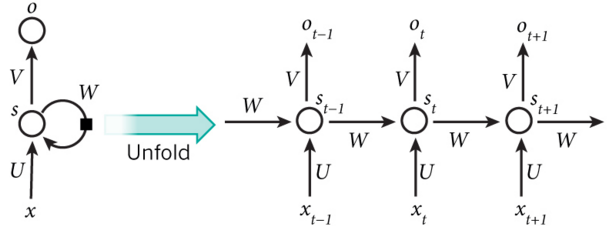
\includegraphics[width=\linewidth]{Images/rnn.PNG}
    \caption{Ontrolling van een recurrent neuraal netwerk}
    \label{fig:rnn}
\end{figure}

Het voorspellen van een zin met een RNN gebeurt woord per woord. Op basis van de eerder waargenomen woorden kan een softmax laag een kansverdeling maken voor het volgende woord. Met behulp van beam-search of het samplen van het meest waarschijnlijke woord, is het netwerk in staat om zinnen te genereren. Tijdens de trainingsfase worden woorden in de vorm van een vector aan het netwerk gegeven. Deze vectoren kunnen gebaseerd zijn op one-hot codering, ze kunnen random zijn, of het kunnen word embeddings zijn zoals bijvoorbeeld \texttt{word2vec}\cite{Mikolov2013}. Deze codering van woorden tot vectoren zelf kan ook deel uitmaken van het netwerk. Als dit het geval is, kan de codering verbeteren tijdens de training met behulp van terugpropagatie \todo{concreet zeggen hoe dit gebeurt}.

\todo{Problemen met RNN: dropout, er is ene goeie paper die vier toevoegingen doet}

% LSTM
\subsection{Long Short Term Memory Neurale Netwerken}
\label{sub:lstm}
Long Short Term Memory (LSTM) is een vorm van RNN die geheugencellen bevat. Door deze cellen is het netwerk in staat om op lange termijn informatie over de input bij te houden. Elk LSTM blok heeft een aantal gates om te bepalen of de input moet onthouden worden, en of een vorige waarde moet bijgehouden of vergeten worden. De output van de cellen is bijgevolg afhankelijk van alle eerder geobserveerde inputs. Figuur \ref{fig:lstm} toont hoe een LSTM-blok er uitziet.\cite{Google}\cite{SeppHochreiter1997}

\begin{figure}[tb]
    \centering
    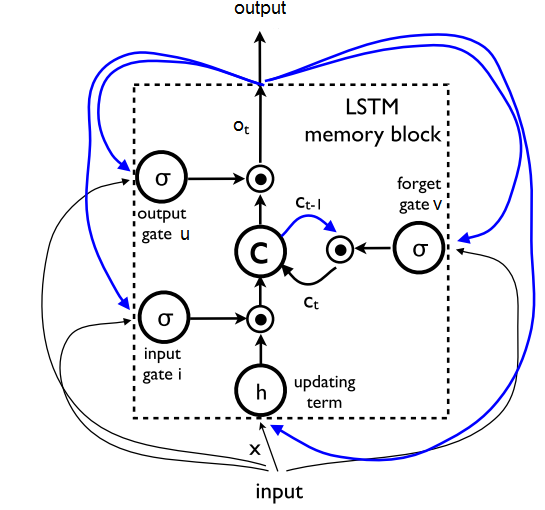
\includegraphics[width=\linewidth]{Images/lstm.PNG}
    \caption{Long Short Term Memory geheugenblok}
    \label{fig:lstm}
\end{figure}

\begin{eqnarray}
\vspace{-3mm}
\label{glstm-memory-start}
i_t' & = & \sigma (W_{ix} x_t + W_{im} m_{t-1}) \label{glstm-input} \\
f_t' & = & \sigma (W_{fx} x_t + W_{fm} m_{t-1}) \\
o_t' & = & \sigma (W_{ox} x_t + W_{om} m_{t-1}) \\
c_t' & = & f_t' \odot c_{t-1}' + i_t' \odot h(W_{cx} x_t + \nonumber \\
&   & + W_{cm} m_{t-1}) \\
m_t & = & o_t' \odot c_t'\\
p_{t+1} = SoftMax(m_t)
\label{glstm-memory}
\vspace{-3mm}
\end{eqnarray}
\todo[inline]{figuur uitleggen, formules bij methodology}

LSTM-netwerken worden net als RNN gebruikt als taalmodellen en zorgen over het algemeen voor hogere kwaliteit. Dit komt doordat LSTM-netwerken over een langere periode dan een gewoon RNN informatie kan onthouden. Dit maakt het modelleren van sequenties met events, die gescheiden zijn door een langere periode, mogelijk.


\section{Statistiek}

% LDA
\subsection{Latent Dirichlet Allocation}
Latent Dirichlet Allocation\cite{Blei2012} is een generatief probabilistisch model voor discrete data. E\'en van de meest gebruikte toepassingen hiervan is het modelleren van een een verdeling van onderwerpen in een set van tekstdocumenten. Dit concept veronderstelt dat elk document een zekere kansverdeling heeft over alle mogelijke onderwerpen. Deze onderwerpen hebben op hun beurt een kansverdeling over alle mogelijke woorden. Zo beschrijft formule \ref{formule:lda} de kans dat een bepaald document $d_j$ een bepaald woord $w_i$ bevat. 

\begin{equation}
    P(w_i | d_j) = \sum\limits_{k=0}^{n_{topics}}P(w_i|topic_k)P(topic_k|d_j)
    \label{formule:lda}
\end{equation}

Een  \ref{fig:lda}. Op basis van twee Dirichlet priors $\alpha$ en $\beta$ word een kansverdeling over de onderwerpen gesampled per document ($\theta$), alsook een kansverdeling over de woorden voor elk onderwerp ($\phi$). Uit $\theta$ wordt voor elke positie $i$ in een document $j$ een onderwerp gesampled ($z_{ji}$). Het samplen van de woordverdeling voor dit onderwerp leidt tot het woord $w_{ji}$. Trainen van een LDA model gebeurt met een Markov chain Monte Carlo algoritme zoals bijvoorbeeld Gibbs sampling, en leidt tot de verdelingen $\theta$ en $\phi$. \todo{herschrijven}

Het trainen met Gibbs sampling begint met een random initialisatie van de topicverdeling voor elk document. Daarna itereert het algoritme over elk woord in elk document. Het berekent de kansverdeling over de verschillende topics, gebaseerd op de onderwerpen van de andere woorden in de collectie (update stap). Op basis van deze kansverdeling wordt een nieuw topic gesampled voor het huidige woord. Dit proces van updaten en samplen herhaalt zich tot er convergentie plaatsvindt. De geleerde topicverdelingen voor elk woord dienen dan als basis voor de topicverdelingen voor elk document en de woordverdelingen per topic. \todo{E en M formules toevoegen}

Het meest interessante voor deze masterproef zijn de topicverdelingen per document. Deze kunnen gebruikt worden als extra semantische informatie. De systemen kunnen op basis van dergelijke topicverdelingen een verband leren tussen de topics die voorkomen in de beschrijvingen, en de concepten die aanwezig zijn op de afbeelding. 
\todo[inline]{formules ook? is natuurlijk mooi, maar meer symbolen, en mss iets overkill?}
\todo[inline]{wat is mcmc, wat zijn dirichlet priors?} 
\todo[inline]{generative story toevoegen}
\begin{figure}[tb]
    \centering
    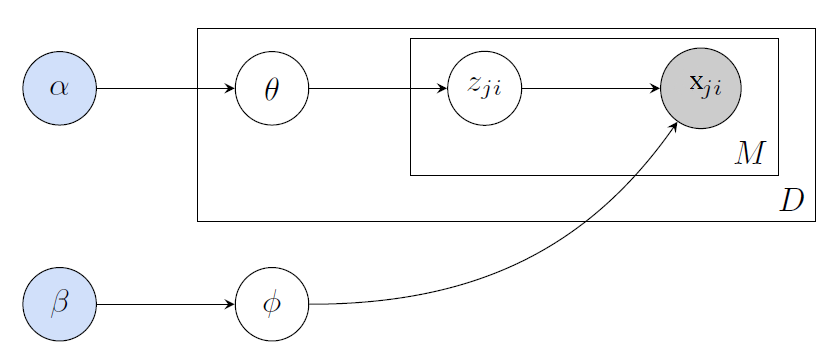
\includegraphics[width=\linewidth]{Images/lda.png}
    \caption{Grafische weergave van LDA}
    \label{fig:lda}
\end{figure}


%  Stacked CCA
\subsection{Canonical Correlation Analysis}
\label{sub:stackedcca}
Canonical Correlation Analysis (CCA) is een methode die gebruikt wordt om een covariantiematrix van twee datasets te berekenen. Dit houdt in dat er een projectie wordt gemaakt naar een gemeenschappelijke ruimte voor beide datasets. De projecties van overeenkomstige waarden zijn na berekening van de modellen maximaal gecorreleerd. In het onderzoek naar image captioning kan dit bijvoorbeeld leiden tot een multimodale mapping van afbeeldings- en beschrijvingsrepresentatie.
\todo[inline]{Referentie voor CCA} \todo{Iets over de training?, hoe wordt dit berekend?}

\paragraph{Stacked CCA}

Stacked Auxiliary Embedding\cite{Gong2014} kan op basis van extra informatie een verbeterde mapping maken. Een voorbeeld hiervan is een dataset van geannoteerde foto's, versterkt met per foto een set van stukjes van de foto met een bijbehorende beschrijving. De representaties van de foto's en annotaties uit de dataset kunnen verbeterd worden door gebruik te maken van de informatie uit de extra dataset.
\todo{DUIDELIJK zeggen dat we van gong stelen}

Om de uiteindelijke augmentatie te bereiken, zijn er een aantal stappen nodig. Uit de extra dataset volgt een eerste set van CCA projecties ($A$, $B$). Daarna volgt een projectie van de originele dataset ($X$, $Y$) naar de multimodale ruimte, door vermenigvuldiging met $A$ en $B$, resulterend in projecties $AX$ en $BY$. Vervolgens transformeren we $AX$ en $BY$ volgens de niet-lineaire functie $\phi(x)$, zoals voorgesteld in de originele paper.

Concatenatie van de originele dataset met het resultaat van de niet-lineaire transformatie leidt tot $\hat{X} = [X, \phi(XA)], \hat{Y} = [Y, \phi(YB)]$. Een laatste stap in het proces is het berekenen van een CCA projectie die gebaseerd is op $\hat{X}$ en $\hat{Y}$, wat resulteert in $U$ en $V$.

Om de dimensionaliteit van de projectie te verhogen wordt voor $\phi(x)$ een random Fourier Feature (RFF) mapping gebruikt. Deze RFF is een functie gebaseerd op de gemiddelde afstand tot de vijftigste dichtste buur van de inputvector. Voor elke foto en caption wordt gekeken welke andere foto of caption de vijftigste dichtste buur is, om vervolgens het gemiddelde te nemen van alle afstanden. De exacte berekening is $\phi(\mathbf{x})=\sqrt{2}cos(\mathbf{x}R+\mathbf{b})$. Hierin is $R$ een matrix die verkregen wordt door sampling van een normaalverdeling met gemiddelde 0, en standaardafwijking $\sigma^2$, waarbij $\sigma$ overeen komt met de eerder berekende gemiddelde afstand. Vector $b$ is resultaat van sampling uit een uniforme verdeling [0,1].

De projectie van een ongeziene afbeelding is het resultaat van het achtereenvolgens uitvoeren van alle transformaties. Voor vector $\mathbf{x}$ geeft dit $\mathbf{\hat{x}} = U[\mathbf{x}, \phi(A\mathbf{x})]$. Deze representatie kan gebruikt worden als een verbeterde versie van de originele image vector, bijvoorbeeld bij een image retrieval taak.
